\scanpage{10}
% Consolidated by root from three independent readings and seventeen adjudication crops.
% crop-candidate: scan 10
\figure{%
\begin{tikzpicture}[x=.0056cm,y=-.0056cm,line cap=round,line join=round,line width=.57pt,
 every node/.style={font=\scriptsize,inner sep=1pt}]
% Upper row. Coordinates follow the scans, with y increasing toward the foot.
\draw (118,180) .. controls (96,175) and (65,165) .. (63,146) .. controls (60,125) and (74,98) .. (94,68) .. controls (114,54) and (139,53) .. (158,62) .. controls (185,75) and (200,102) .. (186,137) .. controls (174,168) and (147,184) .. (118,180) -- cycle;
\draw (80,83) .. controls (88,71) and (96,67) .. (99,65);
\draw (136,55) .. controls (127,87) and (124,146) .. (117,181);
\draw (318,164) .. controls (303,149) and (280,133) .. (288,110) .. controls (294,84) and (305,65) .. (324,65) .. controls (344,61) and (369,61) .. (385,78) .. controls (402,97) and (402,127) .. (387,146) .. controls (369,166) and (333,176) .. (318,164) -- cycle;
\draw (304,85)--(313,65) (292,83) .. controls (303,69) and (310,78) .. (316,72);
\draw (359,63) .. controls (347,100) and (337,144) .. (319,163);
\draw (386,75) .. controls (376,99) and (355,139) .. (359,165);
\draw (528,88) .. controls (548,68) and (579,74) .. (590,94) .. controls (606,122) and (591,152) .. (572,164) .. controls (549,174) and (523,169) .. (512,155) .. controls (495,128) and (504,101) .. (528,88) -- cycle;
\draw (505,107) .. controls (512,94) and (526,94) .. (530,85);
\draw (527,88) -- (544,125) -- (563,157);
\draw (512,158) -- (544,125) -- (579,82);
\fill (545,125) circle[radius=7.5];
\node at (568,39) {OK};
\draw (714,165) .. controls (692,138) and (707,102) .. (741,82) .. controls (763,71) and (805,69) .. (824,85) .. controls (845,101) and (838,140) .. (811,169) .. controls (783,190) and (740,190) .. (714,165) -- cycle;
\draw (750,82) .. controls (741,112) and (733,154) .. (716,171);
\draw (789,74) .. controls (771,116) and (760,159) .. (758,188);
\draw (821,83) .. controls (812,113) and (798,150) .. (809,171);
\draw (774,82) -- (788,74);
\draw (877,167) .. controls (874,143) and (884,111) .. (899,102) .. controls (914,94) and (943,93) .. (957,104) .. controls (971,119) and (978,145) .. (968,163) .. controls (951,183) and (921,193) .. (898,188) .. controls (882,184) and (875,177) .. (877,167) -- cycle;
\draw (899,101) .. controls (909,128) and (902,148) .. (877,166);
\draw (934,99) .. controls (946,117) and (947,134) .. (977,137);
\draw (898,186) .. controls (925,163) and (946,151) .. (968,162);
\draw (925,98)--(927,104) (934,98)--(940,106);
\draw (1007,168) .. controls (1007,137) and (1016,107) .. (1031,102) .. controls (1052,96) and (1065,106) .. (1066,128) .. controls (1065,157) and (1048,186) .. (1027,195) .. controls (1016,201) and (1009,184) .. (1007,168) -- cycle;
\draw (1015,118) -- (1031,130) -- (1063,132) (1008,170) -- (1032,129) -- (1057,103);
\draw (1015,194) .. controls (1031,167) and (1054,156) .. (1054,176);
\fill (1033,130) circle[radius=5.3];
\draw (1038,111)--(1055,103);
\draw (1089,170) .. controls (1094,140) and (1114,106) .. (1137,93) .. controls (1161,77) and (1199,88) .. (1222,101) .. controls (1246,124) and (1228,161) .. (1207,184) .. controls (1180,207) and (1144,214) .. (1121,202) .. controls (1102,193) and (1091,184) .. (1089,170) -- cycle;
\draw (1086,171) -- (1137,135) -- (1167,113) -- (1196,92);
\draw (1119,103) -- (1138,135) .. controls (1151,149) and (1170,178) .. (1184,195);
\draw (1156,86) .. controls (1161,103) and (1168,122) .. (1179,137) .. controls (1195,152) and (1201,165) .. (1217,172);
\draw[line width=3pt] (1138,135) -- (1167,113);
\node at (1153,55) {OK};
\draw (1306,198) .. controls (1298,178) and (1312,140) .. (1333,113) .. controls (1351,93) and (1383,82) .. (1400,89) .. controls (1420,98) and (1435,120) .. (1430,147) .. controls (1413,188) and (1379,216) .. (1344,216) .. controls (1326,214) and (1312,207) .. (1306,198) -- cycle;
\draw (1317,195)--(1397,89) (1328,115)--(1425,174) (1297,172) .. controls (1340,167) and (1385,161) .. (1436,139);
\fill (1338,166)--(1363,135)--(1394,153)--cycle;
\draw[line width=2pt] (1376,90) .. controls (1385,86) and (1397,86) .. (1404,94);
\node at (1376,52) {OK};
\draw (1490,75) .. controls (1477,75) and (1450,148) .. (1446,194) .. controls (1442,229) and (1454,246) .. (1486,240);
\node at (1495,165) {ou};
\draw (1554,177) .. controls (1552,150) and (1562,112) .. (1579,106) .. controls (1599,99) and (1624,111) .. (1633,135) .. controls (1642,163) and (1621,194) .. (1600,205) .. controls (1579,218) and (1555,209) .. (1554,177) -- cycle;
\draw (1566,129) .. controls (1578,149) and (1590,162) .. (1618,175);
\draw (1583,104) .. controls (1582,132) and (1587,174) .. (1597,205);
\draw (1568,206)--(1613,107);
\draw (1567,184) .. controls (1567,196) and (1567,206) .. (1571,209);
\draw[line width=1pt] (1592,178) .. controls (1591,196) and (1590,217) .. (1587,238);
\fill (1587,159) circle[radius=6.5];
% Detached dark fragments beside the lower descending stroke; role uncertain.
\draw[line width=.7pt] (1596,174)--(1595,180) (1595,182)--(1593,187);
\fill (1584,198) circle[radius=1.2]; \fill (1598,226) circle[radius=1.2];
\draw[opacity=.45] (1548,116) .. controls (1562,103) and (1574,101) .. (1584,102);
\draw (1632,96) .. controls (1647,66) and (1657,114) .. (1649,157) .. controls (1641,212) and (1624,259) .. (1606,273);
\draw (759,202) .. controls (780,226) and (799,220) .. (828,212) .. controls (843,208) and (846,205) .. (846,217) .. controls (872,197) and (918,220) .. (949,210) -- (944,207);
\draw[line width=.55pt] (746,274) .. controls (747,244) and (777,229) .. (821,226) .. controls (863,222) and (910,214) .. (923,230) .. controls (940,253) and (888,293) .. (840,300) .. controls (787,310) and (751,304) .. (746,282) -- cycle;
\draw[line width=.7pt] (949,271) .. controls (947,245) and (987,240) .. (1015,235) .. controls (1044,226) and (1072,217) .. (1068,255) .. controls (1064,295) and (1053,303) .. (1014,305) .. controls (969,310) and (951,299) .. (949,271) -- cycle;
\node[inner sep=0pt] at (121,235) {\begin{minipage}{75pt}
\diagram{\begin{tikzcd}[ampersand replacement=\&,column sep=4pt,row sep=0pt,cells={nodes={inner sep=0pt,outer sep=0pt}}]
\bullet
\end{tikzcd}}
\end{minipage}};
\node[inner sep=0pt] at (325,236) {\begin{minipage}{75pt}
\diagram{\begin{tikzcd}[ampersand replacement=\&,column sep=4.7pt,row sep=0pt,cells={nodes={inner sep=0pt,outer sep=0pt}}]
\bullet \& \bullet
\end{tikzcd}}
\end{minipage}};
\node[inner sep=0pt] at (533,233) {\begin{minipage}{75pt}
\diagram{\begin{tikzcd}[ampersand replacement=\&,column sep=13pt,row sep=0pt,cells={nodes={inner sep=0pt,outer sep=0pt}}]
\vphantom{\bullet}\arrow[r,dash,line width=.65pt,start anchor=center,end anchor=center,shorten <=1pt,shorten >=1pt] \& \vphantom{\bullet}
\end{tikzcd}}
\end{minipage}};
\node[inner sep=0pt] at (852,253) {\begin{minipage}{75pt}
\diagram{\begin{tikzcd}[ampersand replacement=\&,column sep=8pt,row sep=0pt,cells={nodes={inner sep=0pt,outer sep=0pt}}]
\bullet \& \bullet \& \bullet
\end{tikzcd}}
\end{minipage}};
\node[inner sep=0pt] at (1009,262) {\begin{minipage}{75pt}
\diagram{\begin{tikzcd}[ampersand replacement=\&,column sep=4pt,row sep=0pt,cells={nodes={inner sep=0pt,outer sep=0pt}}]
\vphantom{\bullet}\arrow[r,dash,line width=.65pt,start anchor=center,end anchor=center,shorten <=1pt,shorten >=1pt] \&[5.2pt] \vphantom{\bullet} \&[-2pt] \bullet
\end{tikzcd}}
\end{minipage}};
\node[inner sep=0pt] at (1152,251) {\begin{minipage}{75pt}
\diagram{\begin{tikzcd}[ampersand replacement=\&,column sep=8.3pt,row sep=0pt,cells={nodes={inner sep=0pt,outer sep=0pt}}]
\bullet\arrow[r,dash,line width=.65pt,start anchor=center,end anchor=center,shorten <=1pt,shorten >=1pt] \& \unsure{\bullet|\circ}\arrow[r,dash,line width=.65pt,start anchor=center,end anchor=center,shorten <=2.7pt,shorten >=1pt] \& \bullet
\end{tikzcd}}
\end{minipage}};
\node[inner sep=0pt] at (1326,262) {\begin{minipage}{75pt}
\diagram{\begin{tikzcd}[ampersand replacement=\&,column sep=1.2pt,row sep=2.0pt,cells={nodes={inner sep=0pt,outer sep=0pt}}]
{} \& \bullet\arrow[dl,dash,line width=.65pt]\arrow[dr,dash,line width=.65pt] \& {}\\
\bullet\arrow[rr,dash,line width=.65pt] \& {} \& \bullet
\end{tikzcd}}
\end{minipage}};
% Two small, detached ink traces near the upper edge.
% Detached upper-edge marks: their hand and function remain undetermined.
\draw[opacity=.65,line width=.55pt] (1018,26) .. controls (1020,31) and (1023,32) .. (1025,27);
\draw[opacity=.65,line width=.55pt] (1037,29)--(1037,26) .. controls (1040,28) and (1043,28) .. (1046,25)--(1046,28);
% Middle row, left group.
\draw (116,390) .. controls (129,357) and (164,337) .. (200,327) .. controls (226,322) and (254,320) .. (272,326) .. controls (307,338) and (328,377) .. (326,413) .. controls (324,455) and (301,485) .. (265,500) .. controls (239,512) and (207,515) .. (184,510) .. controls (147,506) and (125,480) .. (116,455) .. controls (111,433) and (112,411) .. (116,390) -- cycle;
\draw (122,399) .. controls (122,392) and (126,388) .. (131,388);
\draw (154,353) .. controls (158,379) and (146,454) .. (128,472);
\draw (205,327) .. controls (203,354) and (205,404) .. (201,431) .. controls (197,465) and (193,491) .. (191,513);
\draw (270,324) .. controls (258,366) and (252,404) .. (253,433) .. controls (252,456) and (256,486) .. (263,501);
\draw (311,367) .. controls (296,393) and (290,441) .. (305,475);
\draw[opacity=.2] (192,503)--(195,556);
\draw (400,505) .. controls (378,492) and (374,467) .. (377,444) .. controls (382,413) and (403,377) .. (420,364) .. controls (441,342) and (462,334) .. (482,340) .. controls (514,337) and (544,366) .. (542,403) .. controls (543,444) and (508,491) .. (484,503) .. controls (462,516) and (428,521) .. (400,505) -- cycle;
\draw (419,365) .. controls (426,377) and (409,469) .. (400,503);
\draw (482,343) .. controls (461,390) and (451,446) .. (449,510);
\draw (517,356) .. controls (502,397) and (484,451) .. (481,501);
\draw[line width=1.6pt] (406,503) .. controls (423,481) and (428,504) .. (433,517);
\draw (433,512)--(434,519) (448,491)--(447,513) (456,346)--(482,340);
\draw (568,459) .. controls (563,432) and (570,399) .. (581,379) .. controls (594,358) and (612,345) .. (640,352) .. controls (665,358) and (685,385) .. (687,411) .. controls (693,446) and (680,490) .. (647,519) .. controls (636,523) and (624,523) .. (609,524) .. controls (590,517) and (571,499) .. (568,480) -- cycle;
\draw (598,359) .. controls (613,387) and (599,433) .. (567,459);
\draw (645,353) .. controls (653,386) and (676,407) .. (693,410);
\draw (570,480) .. controls (590,487) and (605,503) .. (610,524);
\draw[line width=1pt] (644,519) .. controls (647,504) and (665,473) .. (682,462);
\draw[line width=1.8pt] (684,395) .. controls (697,432) and (683,488) .. (651,516);
\draw (178,557) .. controls (177,574) and (221,577) .. (266,570) .. controls (311,564) and (361,554) .. (376,584) .. controls (378,560) and (416,560) .. (439,563) .. controls (497,573) and (539,558) .. (631,549);
\fill (733,427) circle[radius=2]; \fill (713,443) circle[radius=1.1];
% Middle row, right group.
\draw (778,444) .. controls (795,393) and (841,368) .. (889,367) .. controls (926,365) and (959,385) .. (977,414) .. controls (1001,449) and (966,489) .. (944,514) .. controls (923,544) and (901,563) .. (874,562) .. controls (842,564) and (800,553) .. (774,526) .. controls (774,509) and (771,472) .. (778,444) -- cycle;
\draw (772,446) .. controls (815,439) and (889,422) .. (947,388);
\draw (790,536) -- (854,425) -- (891,367);
\draw (778,464) .. controls (801,466) and (800,495) .. (777,509);
\draw (909,368) .. controls (910,392) and (925,388) .. (937,375);
\draw (774,517) .. controls (783,516) and (781,535) .. (791,536);
\fill (855,425) circle[radius=7.6];
\draw (990,500) .. controls (989,465) and (1002,432) .. (1026,409) .. controls (1047,386) and (1072,381) .. (1088,394) .. controls (1114,409) and (1110,444) .. (1104,473) .. controls (1098,508) and (1073,550) .. (1052,568) .. controls (1023,582) and (1009,571) .. (1000,548) .. controls (994,529) and (990,511) .. (990,500) -- cycle;
\draw (1021,412) .. controls (1043,438) and (1062,481) .. (1078,517);
\draw (998,534) .. controls (1023,505) and (1065,431) .. (1091,399);
\draw (998,456) .. controls (1018,463) and (1009,490) .. (991,501);
\draw (1015,570) .. controls (1034,544) and (1052,547) .. (1057,562);
\fill (1053,458) ellipse[x radius=6.8,y radius=9];
\draw (1133,512) .. controls (1136,476) and (1157,427) .. (1183,402) .. controls (1209,376) and (1248,380) .. (1268,395) .. controls (1296,420) and (1293,459) .. (1285,493) .. controls (1274,530) and (1241,562) .. (1208,571) .. controls (1171,582) and (1146,555) .. (1137,534) .. controls (1133,523) and (1132,516) .. (1133,512) -- cycle;
\draw (1172,411) -- (1207,472) .. controls (1222,498) and (1233,526) .. (1243,551);
\draw (1144,552) .. controls (1161,534) and (1218,450) .. (1266,395);
\draw (1155,453) .. controls (1175,478) and (1159,506) .. (1133,523);
\draw (1159,444) .. controls (1166,453) and (1181,440) .. (1171,428);
\fill (1207,472) circle[radius=7.3];
\draw (1285,514) .. controls (1291,476) and (1311,437) .. (1337,415) .. controls (1356,400) and (1381,409) .. (1391,423) .. controls (1417,463) and (1404,507) .. (1384,535) .. controls (1369,559) and (1349,583) .. (1327,588) .. controls (1306,591) and (1288,575) .. (1284,550) .. controls (1281,536) and (1282,525) .. (1285,514) -- cycle;
\draw (1315,444) -- (1342,491) -- (1368,559);
\draw (1290,564) .. controls (1307,552) and (1355,466) .. (1388,423);
\draw (1299,575) .. controls (1317,554) and (1335,524) .. (1347,555) -- (1353,570);
\draw (1312,585) .. controls (1328,561) and (1340,561) .. (1340,582);
\fill (1343,492) circle[radius=6.6];
\fill (1307,505) .. controls (1310,497) and (1314,496) .. (1318,483) .. controls (1324,477) and (1329,500) .. (1324,509) .. controls (1317,520) and (1305,515) .. (1307,505) -- cycle;
% Undetermined trace: pale intervals separate the darker parts of this upper extension.
\draw[opacity=.22] (1328,433) .. controls (1330,406) and (1335,357) .. (1341,329);
\draw[line width=.65pt] (1340,332)--(1339,339) (1338,343) .. controls (1336,351) and (1337,359) .. (1335,365);
\draw[line width=.55pt] (1333,382)--(1332,389) (1331,398)--(1330,403) (1329,411)--(1327,432);
\draw[line width=1.8pt] (1327,436) .. controls (1335,425) and (1340,416) .. (1349,418);
\draw (793,583) .. controls (822,621) and (923,616) .. (981,613) .. controls (1025,612) and (1060,623) .. (1079,622) .. controls (1090,628) and (1095,637) .. (1102,649) .. controls (1114,632) and (1127,626) .. (1138,621) .. controls (1220,627) and (1280,619) .. (1348,616) .. controls (1354,610) and (1360,601) .. (1364,592);
\draw (1004,605) .. controls (1015,626) and (1050,615) .. (1069,622) (1167,622) -- (1204,630);
\node[font=\bfseries\small] at (539,658) {?};
\node[inner sep=0pt] at (373,646) {\begin{minipage}{85pt}
\diagram{\begin{tikzcd}[ampersand replacement=\&,column sep=7pt,row sep=0pt,cells={nodes={inner sep=0pt,outer sep=0pt}}]
\bullet \& \bullet \& \bullet \& \bullet
\end{tikzcd}}
\end{minipage}};
\node[inner sep=0pt] at (848,648) {\begin{minipage}{85pt}
\diagram{\begin{tikzcd}[ampersand replacement=\&,column sep=11.1pt,row sep=0pt,cells={nodes={inner sep=0pt,outer sep=0pt}}]
\vphantom{\bullet}\arrow[r,dash,line width=.65pt,start anchor=center,end anchor=center,shorten <=1pt,shorten >=1pt] \& \vphantom{\bullet} \& \bullet \& \bullet
\end{tikzcd}}
\end{minipage}};
% Lower row.
\draw[opacity=.22,line width=.4pt] (1518,375) .. controls (1540,374) and (1561,405) .. (1524,401);
\fill[opacity=.75] (1566,580) circle[radius=1.25]; \fill[opacity=.65] (1561,587) circle[radius=1];
\node at (201,691) {OK};
\draw (123,811) .. controls (135,770) and (168,740) .. (208,726) .. controls (239,716) and (275,725) .. (304,749) .. controls (339,775) and (354,809) .. (350,840) .. controls (347,879) and (314,935) .. (279,960) .. controls (257,972) and (226,969) .. (198,968) .. controls (162,965) and (130,943) .. (121,913) .. controls (114,887) and (118,844) .. (123,811) -- cycle;
\draw (124,893) .. controls (149,863) and (184,800) .. (219,718);
\draw (125,813) -- (194,773) .. controls (223,757) and (257,743) .. (274,727);
\draw (198,968) -- (298,838) -- (340,790);
\draw (277,965) .. controls (283,927) and (291,876) .. (298,839) .. controls (303,812) and (307,781) .. (310,754);
\fill (194,773) circle[radius=7.5]; \fill (299,838) circle[radius=7];
\draw[opacity=.14] (252,825)--(256,825) (259,825)--(264,826) (267,826)--(271,826) (274,827)--(278,827);
\draw[opacity=.4] (278,827)--(293,828);
% State remains uncertain: diagonal cancellation | hatching. Only the visible diagonal paths are inked.
\node[inner sep=0pt,outer sep=0pt,anchor=center] at (548,820) {\unsure{\rlap{\hbox{\begin{tikzpicture}[x=.0056cm,y=-.0056cm,line cap=round,line join=round,line width=.57pt,color=black]
\path[use as bounding box] (450,714) rectangle (646,926);
\draw (460,830) .. controls (473,785) and (509,749) .. (541,731) .. controls (566,724) and (595,741) .. (613,754) .. controls (645,781) and (638,817) .. (626,842) .. controls (605,883) and (571,914) .. (538,917) .. controls (508,924) and (480,912) .. (462,889) .. controls (452,874) and (454,848) .. (460,830) -- cycle;
\draw (474,789) -- (612,754) (461,891) -- (547,729) (556,729) .. controls (578,778) and (605,805) .. (628,838);
% Repeated diagonal cancellation strokes in this disk.
\draw (535,717) .. controls (526,729) and (457,833) .. (461,835) .. controls (470,838) and (538,725) .. (537,729) .. controls (515,764) and (465,860) .. (470,865) .. controls (476,870) and (554,747) .. (565,747) .. controls (549,777) and (493,861) .. (493,865) .. controls (504,870) and (569,753) .. (585,751) .. controls (557,783) and (513,860) .. (518,866) .. controls (526,877) and (601,791) .. (614,798) .. controls (618,801) and (589,843) .. (563,892) .. controls (554,907) and (560,914) .. (572,923);
% Small pale descending trace and dark tip at the lower-left outline.
\draw[opacity=.16,line width=.4pt] (490,861) .. controls (488,885) and (490,901) .. (491,915);
\draw[line width=.55pt] (491,912)--(490,920);
\end{tikzpicture}}}\phantom{\deleted{\hbox{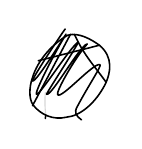
\begin{tikzpicture}[x=.0056cm,y=-.0056cm,line cap=round,line join=round,line width=.57pt,color=black]
\path[use as bounding box] (450,714) rectangle (646,926);
\draw (460,830) .. controls (473,785) and (509,749) .. (541,731) .. controls (566,724) and (595,741) .. (613,754) .. controls (645,781) and (638,817) .. (626,842) .. controls (605,883) and (571,914) .. (538,917) .. controls (508,924) and (480,912) .. (462,889) .. controls (452,874) and (454,848) .. (460,830) -- cycle;
\draw (474,789) -- (612,754) (461,891) -- (547,729) (556,729) .. controls (578,778) and (605,805) .. (628,838);
% Repeated diagonal cancellation strokes in this disk.
\draw (535,717) .. controls (526,729) and (457,833) .. (461,835) .. controls (470,838) and (538,725) .. (537,729) .. controls (515,764) and (465,860) .. (470,865) .. controls (476,870) and (554,747) .. (565,747) .. controls (549,777) and (493,861) .. (493,865) .. controls (504,870) and (569,753) .. (585,751) .. controls (557,783) and (513,860) .. (518,866) .. controls (526,877) and (601,791) .. (614,798) .. controls (618,801) and (589,843) .. (563,892) .. controls (554,907) and (560,914) .. (572,923);
% Small pale descending trace and dark tip at the lower-left outline.
\draw[opacity=.16,line width=.4pt] (490,861) .. controls (488,885) and (490,901) .. (491,915);
\draw[line width=.55pt] (491,912)--(490,920);
\end{tikzpicture}}}}}};
\draw (666,836) .. controls (669,808) and (686,789) .. (706,785) .. controls (725,782) and (746,786) .. (755,803) .. controls (773,824) and (771,857) .. (758,880) .. controls (746,903) and (728,917) .. (706,910) .. controls (683,903) and (660,871) .. (666,836) -- cycle;
\draw (707,786) -- (694,902) (747,789) .. controls (739,827) and (735,869) .. (729,906);
\draw (666,840)--(767,844);
\draw[line width=3.4pt] (699,838)--(737,842);
\draw (718,786) .. controls (715,814) and (733,813) .. (737,789);
\draw (797,850) .. controls (804,822) and (821,801) .. (839,798) .. controls (864,797) and (876,815) .. (881,839) .. controls (890,866) and (876,895) .. (860,910) .. controls (841,926) and (822,917) .. (809,905) .. controls (796,890) and (792,870) .. (797,850) -- cycle;
\draw (827,805) .. controls (823,843) and (819,878) .. (816,915);
\draw (862,805) .. controls (858,842) and (854,879) .. (852,914);
\draw (799,861)--(890,859); \draw[line width=2.8pt] (820,857)--(853,857);
\draw (874,818) .. controls (868,841) and (868,848) .. (885,850);
\draw (543,948) .. controls (573,976) and (607,963) .. (665,954) .. controls (706,949) and (731,945) .. (741,967) .. controls (744,947) and (789,945) .. (826,944) .. controls (864,943) and (881,941) .. (899,937) -- (898,931);
\node at (1156,724) {OK};
\draw (1004,849) .. controls (1005,815) and (1033,783) .. (1069,769) .. controls (1101,757) and (1134,762) .. (1150,787) .. controls (1172,815) and (1183,855) .. (1165,903) .. controls (1149,943) and (1125,964) .. (1109,969) .. controls (1072,976) and (1040,970) .. (1024,945) .. controls (1004,913) and (997,879) .. (1004,849) -- cycle;
\draw[opacity=.65] (1006,850) .. controls (1002,859) and (1003,869) .. (1009,874);
\draw (1012,924) .. controls (1029,875) and (1050,817) .. (1070,770);
\draw (1011,808) .. controls (1055,804) and (1125,796) .. (1156,788);
\draw (1101,764) .. controls (1110,780) and (1116,791) .. (1120,798) -- (1174,881);
\draw (1109,967) .. controls (1127,926) and (1154,855) .. (1172,823);
\draw[line width=2.7pt] (1056,802)--(1119,794);
\draw[line width=3.7pt] (1118,795)--(1158,853);
% Detached short dark trace below the broad segment; role and hand undetermined.
\draw[line width=.55pt] (1166,875)--(1165,879);
% Detached pale irregular patch; hand, origin and role remain undetermined.
\filldraw[fill opacity=.10,draw opacity=.16,line width=.3pt]
(1629,793) .. controls (1629,790) and (1631,788) .. (1635,788)
--(1636,786)--(1640,790)--(1645,792)
.. controls (1649,795) and (1648,799) .. (1646,802)
--(1643,803)--(1640,806)--(1637,808)--(1634,804)--(1630,804)
.. controls (1627,801) and (1627,797) .. (1629,793)--cycle;
% Two faint, angular lines at the foot, crossing the last graph and continuing at the right.
\draw[opacity=.55] (1010,975) .. controls (1027,995) and (1035,1030) .. (1044,1050) .. controls (1053,1074) and (1061,1090) .. (1075,1089);
\draw[line width=1.5pt] (1041,1036) .. controls (1052,1070) and (1060,1090) .. (1074,1088);
\draw[opacity=.16] (1073,1088) .. controls (1108,1087) and (1162,1076) .. (1214,1064) -- (1288,985);
\draw[opacity=.5] (1215,1073)--(1237,1044) (1246,1033)--(1261,1014) (1278,996)--(1289,982);
\draw[opacity=.22] (1345,934) .. controls (1353,954) and (1350,994) .. (1358,1009) -- (1372,1014);
\draw[line width=1.9pt] (1373,1014) .. controls (1390,1025) and (1430,1037) .. (1458,1048) -- (1484,1054) -- (1500,1036);
\draw[opacity=.5] (1487,1054)--(1581,957);
\draw[opacity=.23] (1568,905) .. controls (1572,924) and (1571,943) .. (1581,957);
\node[inner sep=0pt] at (222,1035) {\begin{minipage}{94pt}
\diagram{\begin{tikzcd}[ampersand replacement=\&,column sep=5.2pt,row sep=0pt,cells={nodes={inner sep=0pt,outer sep=0pt}}]
\unsure{\circ|\bullet}\arrow[r,dash,line width=.65pt,start anchor=center,end anchor=center,shorten <=1pt,shorten >=1pt] \& \circ \& \hspace{3.3pt} \& \bullet\arrow[r,dash,line width=.65pt,start anchor=center,end anchor=center,shorten <=1pt,shorten >=1pt] \& \bullet
\end{tikzcd}}
\end{minipage}};
\node[inner sep=0pt] at (563,1026) {\begin{minipage}{94pt}
\diagram{\begin{tikzcd}[ampersand replacement=\&,column sep=7pt,row sep=0pt,cells={nodes={inner sep=0pt,outer sep=0pt}}]
\unsure{\circ|\bullet}\arrow[r,dash,line width=.65pt,start anchor=center,end anchor=center,shorten <=1pt,shorten >=1pt] \& \bullet\arrow[r,dash,line width=.65pt,start anchor=center,end anchor=center,shorten <=2.7pt,shorten >=1pt] \& \bullet \& \bullet
\end{tikzcd}}
\end{minipage}};
\node[inner sep=0pt] at (1075,1032) {\begin{minipage}{94pt}
\diagram{\begin{tikzcd}[ampersand replacement=\&,column sep=9pt,row sep=0pt,cells={nodes={inner sep=0pt,outer sep=0pt}}]
\unsure{\bullet|\circ}\arrow[r,dash,line width=.65pt,start anchor=center,end anchor=center,shorten <=1pt,shorten >=1pt] \& \bullet\arrow[r,dash,line width=.65pt,start anchor=center,end anchor=center,shorten <=1pt,shorten >=1pt] \& \bullet\arrow[r,dash,line width=.65pt,start anchor=center,end anchor=center,shorten <=1pt,shorten >=1pt] \& \bullet
\end{tikzcd}}
\end{minipage}};

% Hook projecting above/right of the uncertain middle vertex under upper disk 7.
\draw[line width=.65pt] (1153,251) .. controls (1154,245) and (1159,246) .. (1163,252);
% Tiny detached spot just above the outer lower arch in the last middle disk.
\fill (1314,543) circle[radius=1.4];
% Pale detached marks; hand, purpose, and surface origin remain undetermined.
% Above upper disk4 the short course is supported; its faint lower continuation is unresolved.
\draw[opacity=.14,line width=.4pt] (416,241) .. controls (425,250) and (426,260) .. (421,266) .. controls (416,274) and (410,275) .. (403,275);
\draw[opacity=.16,line width=.4pt] (784,42) .. controls (784,49) and (785,55) .. (787,62);
\draw[opacity=.4,line width=.4pt] (786,56)--(786,59);
\draw[opacity=.16,line width=.35pt] (369,743) .. controls (379,751) and (390,762) .. (405,778) -- (415,786);
\draw[opacity=.25,line width=.4pt] (377,751)--(384,758) (390,764)--(393,767);
\draw[opacity=.14,line width=.4pt] (1567,352) .. controls (1570,358) and (1576,360) .. (1580,362);
% Pale diagonal inside the right angular trace, with independently detached lower dash.
% Only the short supported course is reproduced; a farther upper continuation remains unresolved.
\node[anchor=north west,inner sep=0pt,outer sep=0pt] at (1438,978) {\unsure{\hbox{\begin{tikzpicture}[x=.0056cm,y=-.0056cm,line cap=round,color=black]
\path[use as bounding box] (1438,978) rectangle (1504,1039);
\draw[opacity=.13,line width=.4pt] (1444,1037) .. controls (1460,1018) and (1488,989) .. (1500,980);
\end{tikzpicture}}}};
\draw[opacity=.45,line width=.45pt] (1435,1084)--(1437,1093);
% Dark pieces and small detached marks around the upper-right angular-trace endpoint.
\draw[opacity=.75,line width=.45pt] (1568,908)--(1570,917);
\fill[opacity=.65] (1566,921) circle[radius=1.15];
\fill[opacity=.3] (1550,893) circle[radius=1.2];
\fill[opacity=.2] (1603,930) circle[radius=1.6];
\end{tikzpicture}}
% archive sheet number: 9

